\section{Service Delivery}
\label{chap:proposal:delivery}

To implement and validate network applications, third parties require a network environment that reproduces the conditions under which each application is supposed to operate. The role of a testbed is not only to provide such a substrate, i.e. the actual physical network and compute infrastructure, but also to provide the necessary capabilities to configure it for each experiment, according to the requirements of the application and target vertical industry. This requires partitioning the shared infrastructure into isolated logical networks through network slicing, exposed as third-party services that let verticals configure slices tailored to their applications. Moreover, the complete lifecycle of the provisioned slices and their UE should follow widely adopted, accessible data models.

Composing complete experiments, however, requires access to other functionalities. The exposure APIs, monitoring services, and the vertical application itself must all be configured, packaged and deployed for each experiment. These capabilities should be offered as services through a single management and automation platform, traditionally an OSS. Through it, verticals can design, order, and manage services as needed, without manually interacting with the underlying infrastructure components which realize their orchestration. Centralizing the provisioning of experiments in a single platform would also ensure that each experiment is instantiated consistently, so that its results can be reproduced and compared across executions.

With this in mind, vertical clients should be able to access this platform both through a graphical interface and programmatically, via standardized APIs that support automation and integration with external tools. TMF ODA addresses this by defining TMF Open APIs to simplify service design, orchestration, and management, abstracting proprietary management interfaces so network capabilities are offered through standardized, interoperable ones.

The remainder of this section details how such a platform may support the complete lifecycle of an experiment by translating vertical requirements into services that can be provisioned and tested on the testbed.


\subsection{Service Design}
\label{chap:proposal:delivery:design}

Each functionality offered by the testbed should be described by a reusable service specification that defines the service's attributes, relationships, and constraints~\cite{SIDTMF, SID-MODELS-v250-TMF}. Following the \acs{TMF} \acs{SID} model, the proposed design distinguishes between specifications for \acsp{CFS}, which describe the service as perceived by the vertical, and \acsp{RFS}, which describe how it is realized over the underlying resources. Each \acs{CFS} exposes a set of configurable characteristics, so that verticals can parameterize services according to their application without knowledge of how these are realized within the testbed. The resulting specifications must be published in a service catalog, from which verticals can browse and order the available services through \acs{TMF} Open \acsp{API}. The \acs{OSS} should additionally provide a \acs{GUI} that allows verticals to perform these operations without directly interacting with the \acsp{API}.

Service specifications may also reference other specifications, forming composite services. A complete experiment typically requires multiple interdependent services that must be configured and provisioned together, e.g. a network slice and its attached \acs{UE}, or a network application and the \acs{5G} exposure \acsp{API} it consumes. These dependencies should be captured as a bundle of services and offered at different levels of granularity depending on the use case. For example, a network slice and its \acsp{UE} can be offered both as standalone services, to extend an existing experiment, and as a single composite service, to provision a complete environment through a single order. In either case, the system is responsible for maintaining a consistent view of the provisioned resources and their dependencies, ensuring that the relationships between them remain explicitly represented regardless of whether these are provisioned through separate service orders or at different times, e.g. when a \acs{UE} is provisioned as a standalone service and attached to a previously provisioned slice, the resulting relationship shall be registered by the system. 

To support the composition of complete experiments, the service catalog should offer the following suite of services.


\bulletparagraph{\textit{Network Slice}}

The Network Slice service should provision an \acs{NSI} tailored to the vertical's \acs{QoS} requirements, managed as established in Section~\ref{chap:proposal:resource_lifecycle}. Its characteristics should express these requirements through configurable standardized slice attributes.

In particular, the Network slice specification should be derived from the \acs{GSMA} \acs{GST}. As discussed in Section~\ref{sec:slice:lifecycle}, the \acs{GST} defines a common set of attributes to describe a network slice, such as throughput, latency, \acs{UE} density and isolation level, which are assigned concrete values in a \acs{NEST} for a specific use case~\cite{GSMA_GST}. Mapping these attributes to the characteristics of the slice service specification would allow verticals to express their requirements through a standardized vocabulary. The management plane should then translate these characteristics into concrete slice requirements that are delegated to the corresponding network slice management functions, i.e. the \acs{NSMF} and the \acs{NSSMF}, as outlined in Section~\ref{chap:proposal:resource_lifecycle}.


\bulletparagraph{\textit{User Equipment}}

The User Equipment service should transparently register a \acs{UE} with the \acs{5G} network and attach it to a provisioned network slice. The design and management of \acs{5G} \acs{UE} are defined across several \acs{3GPP} specifications, namely 3GPP TS 23.501~\cite{}, 3GPP TS 24.527~\cite{} and 3GPP TS 23.503~\cite{}. However, in contrast to network slices, no common template is standardized or recommended for the definition of a \acs{UE}. Because of this, this dissertation proposes a minimal blueprint for modeling \acs{5G} \acsp{UE}, which is presented in Table~\ref{tab:proposal:delivery:ue-blueprint}.

The blueprint identifies the requested slice for the \acs{UE} via the \acs{SST} and optional \acs{SD} fields. In addition, it specifies the aggregate bitrate limits, as well as optional static addressing for the established \acs{PDU} session. These fields constitute a minimal common set and may be extended with implementation specific parameters required by different \acs{5G} distributions.

\begin{table}[htbp]
    \centering
    \renewcommand\tabularxcolumn[1]{m{#1}}
    \begin{tabularx}{\textwidth}{|
        >{\RaggedRight\arraybackslash}m{\widthof{SessionAmbr : Downlink}}|
        >{\RaggedRight\arraybackslash}X|}
        \hline
        \textbf{\acs{UE} Parameter} & \textbf{Description} \\
        \hline
        Requested\acs{NSSAI} : \acs{SST}  & Slice Service Type that identifies the category of the network slice requested by the \acs{UE} \\
        \hline
        Requested\acs{NSSAI} : \acs{SD}  & Optional Slice Differentiator that, with \acs{SST}, forms the \acs{S-NSSAI} uniquely identifying the slice requested by the \acs{UE} \\
        \hline
        SessionAmbr : Uplink & Maximum bitrate allowed for \acs{UE} uplink traffic \\
        \hline
        SessionAmbr : Downlink & Maximum bitrate allowed for \acs{UE} downlink traffic \\
        \hline
        PduSession : IPv4 & Optional field to request a static IPv4 address for the \acs{UE} \\
        \hline
        PduSession : IPv6 & Optional field to request a static IPv6 address for the \acs{UE} \\
        \hline
    \end{tabularx}
    \caption{\acs{UE} blueprint specification}
    \label{tab:proposal:delivery:ue-blueprint}
\end{table}

As the \acs{UE} is only meaningful for the experiment in the context of a slice, the service should declare an explicit dependency to the Network Slice service. That dependency ensures the slice is active before the \acs{UE} is registered, and that the \acs{UE}’s subscription is removed from the \acs{5G} network when the slice is decommissioned.


\bulletparagraph{\textit{Network Exposure}}

The Network Exposure service should allow experimenters to setup the network exposure interfaces mentioned throughout this document, i.e. the \acs{NEF} and CAMARA \acsp{API}, published and secured through the \acs{CAPIF} framework, as described in Section~\ref{chap:proposal:exposure}. 

These interfaces cannot be deployed independently, in paralell, as they follow a strict dependency chain. \acs{CAPIF} must be available first, as the \acs{NEF} relies on it to publish and secure its \acsp{API}. The CAMARA \acsp{API}, in turn, rely on the \acs{NEF} to process their requests and are exposed through \acs{CAPIF}. Nonetheless, not every experiment requires the full exposure layer constituted by all three components. Thus, such an exposure service should support a configuration without the CAMARA \acsp{API}, for cases where the network application interacts with the \acs{NEF} directly, or relying on an alternative authentication method that does not depend on \acs{CAPIF}, preventing it from being provisioned altogether.

Moreover, depending on the actual \acs{NEF} and CAMARA implementation, the vertical developer should also be able to configure the \acs{API} suites required by the application, including options for simulated or live network behavior.


\bulletparagraph{\textit{Network Observability}}

The Network Observability service should enable the collection of network metrics for the resources of the experiment, i.e. the network slice and its \acsp{UE}. Section~\ref{chap:proposal:observability} identifies passive and active monitoring as the two complementary mechanisms through which these metrics can be obtained.

Since active monitoring introduces additional load on the shared infrastructure, it should be exposed as an optional characteristic, disabled by default. When enabled, experimenters should be able to configure the probing conditions, including the probing frequency (interval), number of probes, payload size, and timeout for each probe. More importantly, this configuration should allow experimenters to specify the target \acsp{UE} through their \acsp{IMSI}, so probing and the collected metrics are restricted to the selected devices. This configuration should also be updatable throughout the experiment, without requiring the service to be redeployed.

The metrics of each experiment, including those continuously gathered through passive monitoring, should be presented to the vertical through dedicated visual dashboards, also delivered as part of this service. As multiple experiments share the same infrastructure, each dashboard should be restricted to the network slice and \acsp{UE} of its experiment. For this, the network slice identifier shall be supplied. Additionally, since new \acsp{UE} may be registered and attached to the slice during the experiment, both the dashboards and the active probes must be updated dynamically to reflect the current state of the devices, including any changes to the \acs{IP} addresses of existing \acsp{UE}.


\bulletparagraph{\textit{Network Application}}

The network application service should be created by the vertical using the testbed's \acs{OSS}. Unlike the previous services, whose specifications are designed and maintained by the testbed operator, network applications are specific to each vertical and must first be designed and onboarded into the service catalog. To this end, the experimenter should provide the deployment artifacts and manifests, according to the orchestrators supported by the testbed.

The network application service specification should also declare its dependencies on the remaining services of the experiment. The exposure \acsp{API} it consumes, the observability stack, the required \acsp{UE} and the connectivity conditions established by the network slice are all necessary prerequisites for the application to operate as intended. Thus, these dependencies should determine the order in which the services of an experiment are provisioned, as addressed in the following subsection.


\subsection{Service Orchestration \& Lifecycle Management}
\label{chap:proposal:delivery:orchestration-lifecycle}

Following the definition of network slice and \acs{5G} \acs{UE} templates, the next step is to establish the workflow for integrating these specifications into a platform that supports their configuration, orchestration and lifecycle management.

This platform pertains to the testbed's \acs{OSS}. Rather than exposing proprietary management interfaces, the \acs{OSS} should rely on open northbound \acsp{API} to enable the interoperable and automated management of \acs{5G} resources (network slice and \acs{UE}), exposure services (\acs{NEF}, CAMARA and \acs{CAPIF}), and overall testbed capabilities to experimenters and external systems. To deliver on this requirement and ensure interoperability, the design of the \acs{OSS} should follow established standardization initiatives, namely \acs{TMF}'s \acs{ODA} and their suite of \acs{TMF} Open \acsp{API}, to capture the client's requirements before forwarding them to the concrete orchestrators responsible for their provisioning, at the southbound. The \acsp{API} required for this purpose are listed in Table~\ref{tab:proposal:delivery:orchestration-lifecycle:tmf-apis}.

\begin{table}[htbp]
    \centering
    \renewcommand\tabularxcolumn[1]{m{#1}}
    \begin{tabularx}{\textwidth}{|
        >{\RaggedRight\arraybackslash}m{\widthof{Inventory Management}}|
        >{\RaggedRight\arraybackslash}X|}
        \hline
        \textbf{\acs{TMF} Open \acs{API}} & \textbf{Purpose / Usage} \\
        \hline
        \acs{TMF} 633 Service\newline Catalog Management & Lifecycle Management of Service Catalog elements. Includes publication \& retrieval of Service Specifications modeling \acs{5G} elements, network exposure, observability, and applications. \\
        \hline
        \acs{TMF} 634 Resource\newline Catalog Management & Lifecycle Management of the underlying Resource Catalog elements. \\
        \hline
        \acs{TMF} 638 Service\newline Inventory Management & Manipulation and querying of the runtime inventory of Service instances across stages (e.g. active, reserved, terminated). \\
        \hline
        \acs{TMF} 639 Resource\newline Inventory Management & Manipulation and querying of the runtime inventory of underlying Resource instances. \\
        \hline
        \acs{TMF} 641 Service\newline Ordering Management & Lifecycle management of Service Orders. Covers the creation, update, retrieval and termination of Service Orders, triggering the fulfillment of the requested Service instances. \\
        \hline
        \acs{TMF} 652 Resource\newline Ordering Management & Lifecycle management of underlying Resource Orders. \\
        \hline
    \end{tabularx}
    \caption{\acs{TMF} Open \acsp{API} required for the service delivery methodology of the testbed}
    \label{tab:proposal:delivery:orchestration-lifecycle:tmf-apis}
\end{table}

Exposing network capabilities to experimenters requires hiding the implementation details of the testbed behind a uniform, operator-facing model. As outlined in Section~\ref{sota:telcoinitiatives:tmf}, the \acs{SID} model that underpins the \acs{TMF} \acs{ODA} architecture, provides such a model, clearly distinguishing between the functionalities that are offered, i.e. the services, from the means used to deliver them, i.e. the resources.

This duality is also present across the full list of \acs{TMF} \acs{API} mentioned above. The service-level \acsp{API} constitute the interface through which verticals should interact with the testbed. In constrast, the resource-level \acsp{API} are not intended to be consumed directly by verticals, but rather to be used by the \acs{OSS} itself when decomposing a service order into the underlying resources required for their realization.

Therefore, the definition of orderable specifications relies on catalog-centric \acsp{API}: the \acs{TMF}~633 (Service Catalog Management) and \acs{TMF}~634 (Resource Catalog Management) \acsp{API}. In particular, the \acs{TMF}~633 \acs{API} exposes the service catalog described in Section~\ref{chap:proposal:delivery:design}, allowing experimenters to discover the available service specifications and their configurable characteristics, while the \acs{TMF}~634 \acs{API} plays the equivalent role for the underlying resource specifications. Combined, these \acsp{API} form an abstraction layer that conceals the complexity of the underlying procedures from the experimenter.

Furthermore, since each specification is essentially a set of typed characteristics, it provides a natural basis for the definition of proposed templates. The parameters of the \acs{GSMA} \acs{GST} (instantiated as a \acs{NEST}), of the \acs{UE} blueprint, or of any other testbed components can be expressed as characteristics of \acs{TMF} service and resource specifications. As a result, network capabilities can be offered through the \acs{OSS} as technology-agnostic services that can be reused across different experiments.

Once designed, services shall be instantiated through service orders submitted to the management platform via the \acs{TMF}~641 (Service Ordering Management) \acs{API}, which triggers the issuance of the corresponding resource orders through the \acs{TMF}~652 (Resource Ordering Management) \acs{API}. These orders should then be decomposed and delegated to the appropriate orchestrators responsible for the deployment of each resource.

Given the heterogeneity of experimentation components, the testbed must support multiple deployment paradigms, accommodating both \acs{NFV} and cloud-native resources by leveraging \acsp{NFVO} and container orchestration platforms such as Kubernetes. In addition, support for custom orchestrators or resource controllers may also be beneficial, allowing experimenters to integrate domain or proprietary components, and expose them through standardized management interfaces. Depending on the underlying \acs{5G} infrastructure, these may include, for instance, the management and provisioning of \acs{5G} resources such as network slices and \acsp{UE}.

The \acs{OSS} is therefore entrusted with this responsibility. This delegation confines the actual deployment and lifecycle management of resources to each orchestrator, while the \acs{OSS} maintains a single, uniform service model across them all. As a result, experimenters can order and manage services in the same way regardless of how they are realized, and new orchestrators or deployment paradigms can be more easily integrated, abstracted by the specifications exposed in the service catalog.

Beyond the deployment of individual services, the provisioning workflow must also account for the dependencies between them. These dependencies determine the order in which services are instantiated and the conditions that must verify before each one can be provisioned. For this reason, the \acs{OSS} must provide a way to declare these dependencies within the service specifications and use them to coordinate the lifecycle of all services in an experiment. During instantiation, services are provisioned in the order their dependencies impose, and each service is only deployed once its prerequisites are active and healthy. Such relationships should also be registered on the inventory, at the level of each service instance. Conversely, when any component fails to be instantiated, the \acs{OSS} must halt the provisioning of any dependent services and report the failure, so that the experiment and the testbed are never left in a partially deployed, inconsistent state.

Section~\ref{chap:proposal:delivery} identified the suite of services required to conduct a complete experiment for a network application using the proposed testbed functionality, and their dependencies. Combining these dependencies yields the provisioning chain depicted in Figure~\ref{proposal:delivery:orchestration-lifecycle}, which organizes the orchestration of the experiment into sequential phases. After the onboarding phase, in which the vertical designs and configures the service bundle of the experiment, the network slice is provisioned and the \acsp{UE} are attached to it, establishing the connectivity on which every subsequent service relies. The monitoring phase would then deploy the observability stack, probes and dashboards, scoped to the slice and \acsp{UE} just provisioned. The exposure phases should follow, provisioning \acs{CAPIF}, the \acs{NEF} and the CAMARA \acsp{API} in the order imposed by their dependency chain, before the vertical application is finally deployed and configured to consume them. Should any phase fail, the \acs{OSS} should refrain from provisioning any subsequent services. Similarly, terminating the experiment should trigger the termination of all provisioned services.

\begin{figure}[htpb]
    \centering
    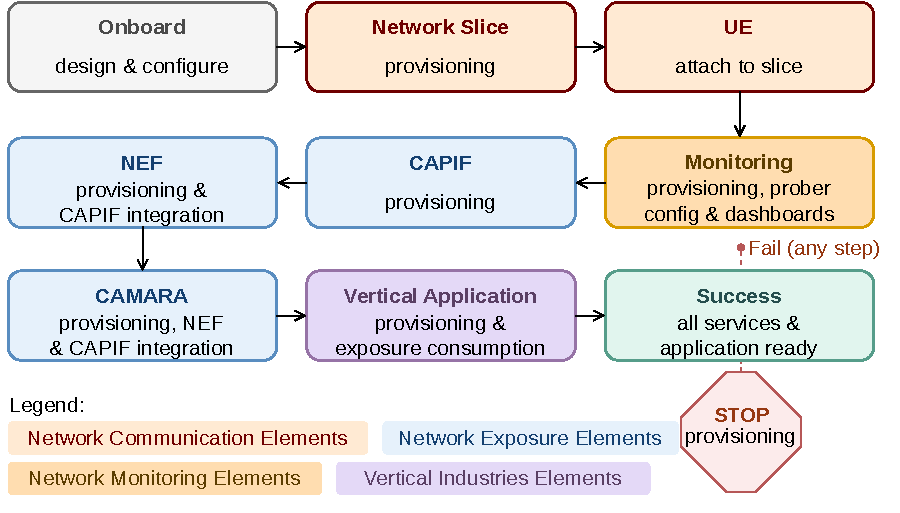
\includegraphics[width=0.8\linewidth]{figs/drawio/service_provisioning_chain.pdf}
    \caption{Sequential Orchestration Phases for a complete Network Application Experiment}
    \label{proposal:delivery:orchestration-lifecycle}
\end{figure}

Lastly, the runtime state of each experiment should be tracked through the \acs{TMF}~638 (Service Inventory Management) and \acs{TMF}~639 (Resource Inventory Management). The service inventory would record each service instance, its state and its relationships to other instances, allowing the \acs{OSS} to identify the dependent services to be created or terminated when an experiment is commissioned or decommissioned. The resource inventory would assume the equivalent role for the underlying resources, confirming that they are allocated on or released from the shared infrastructure.
